\chapter{Future of Wearable Computing}

% Advice: Describe the contributions and how the chapters are linked together (similar to Section 1.5 except more consolidated.  Make statements about applications, significance and how they are all tied together in the framework of humanistic intelligence.  See below for an example, but add more technical terms as you describe the main contributions of the thesis.  Spatiotonal mapping, iCLUT or something!  Maybe even have a bullet list of contributions if appropriate

% Essentially, assume the committee never read anything in your thesis.  What would you like them to know that you did?  Why is this so difficult and important that it is worth a PhD (apart from the fact that this is a fully functional commercial product?  Try to separate that a bit since you want to emphasize what you did before it is commercialized as there will be questions about your own individual contributions if you just focus on "your" product which is really a big teamwork effort to be fair. 

% Also, keep your sentences concise and to the point (Steve's thesis only has 2 pages of conclusion but he had a 200 page thesis)- there's too much reading for someone up to here already if they read your entire thesis.  Summarize, extend, and tell me something new (synthesis of your entire thesis). 

% Need to figure out what to call this: 3-D HDR Aug-mediated Reality Digital Eye Glass?  EyeTap?  Gen-5? 
% I would say let's make this stand out somehow instead of making it sound incremental (Gen-5...?). 
% Similar problem in Ch 1 still - just need consistent terminology 
This thesis proposes the design and practical implementation of a 3D HDR Augmediated Reality Digital Eye Glass system that embodies the principles of humanistic intelligence and extends significantly beyond our human sensory capabilities.  Specifically, the main contributions of this thesis include solving the fundamental limitations of human vision and our sensory capability by extending the dynamic range of the human eye, as demonstrated in the most extreme scenario in tungsten inert gas welding, through real-time 3D stereoscopic HDR management system implemented on both FPGAs and GPUs (\textbf{Chapter~\ref{realtimehdrfpgas}}), and by creating a new form of human-centric computer interaction enabled by a novel form of HDR in space using 3D range sensing cameras (\textbf{Chapter~\ref{3dhdr3dsensing}}) and by a natural gesture input algorithm (\textbf{Chapter~\ref{ar3dgesture}}).  The broader social implications of ubiquitous wearable computing as enabled by the 3-D HDR Augmediated Reality Digital Eye Glass, such as the notion of sousveillance (as opposed to surveillance), were explored in~\textbf{Chapter~\ref{freeglassdevelopers}}. 

% Q: What is anti-gestural input? 
By creating a highly intuitive and portable wearable system that can exceed human capabilities, this platform has become a true extension of the human body and a form of embodied humanistic intelligence.  The final Digital Eye Glass system relies on a tight close feedback loop, in which human and machine work as one entity, thus allowing one to interact with the real world and the virtual world naturally with gestural inputs whereas ultimately the machine can continuously learn from our own action and integrating into our life. The final prototype is an untethered, optical see-through, depth sensor based, and multi-functional wearable system which improves our vision by being able to read distances at millimeter accuracy and navigate freely outdoor under extreme lighting conditions, while being able to perform everyday tasks such as browsing on the web in many social settings.  At one point, I truly felt that I had become a cyborg, and acquired a digital form of superpower, such as night vision, real-time distance measurement, and gestural controls with my bare hands without any accessories.  Finally, the design was successfully translated into a commercial development platform that truly opens up a whole new world of possible augmented reality applications for developers around the world in the near future.

\begin{figure*}
\center
%\includegraphics[width=2in]{ch7/figures/left_white.jpg}
\includegraphics[height=2.8in]{ch7/figures/wearable.jpg}
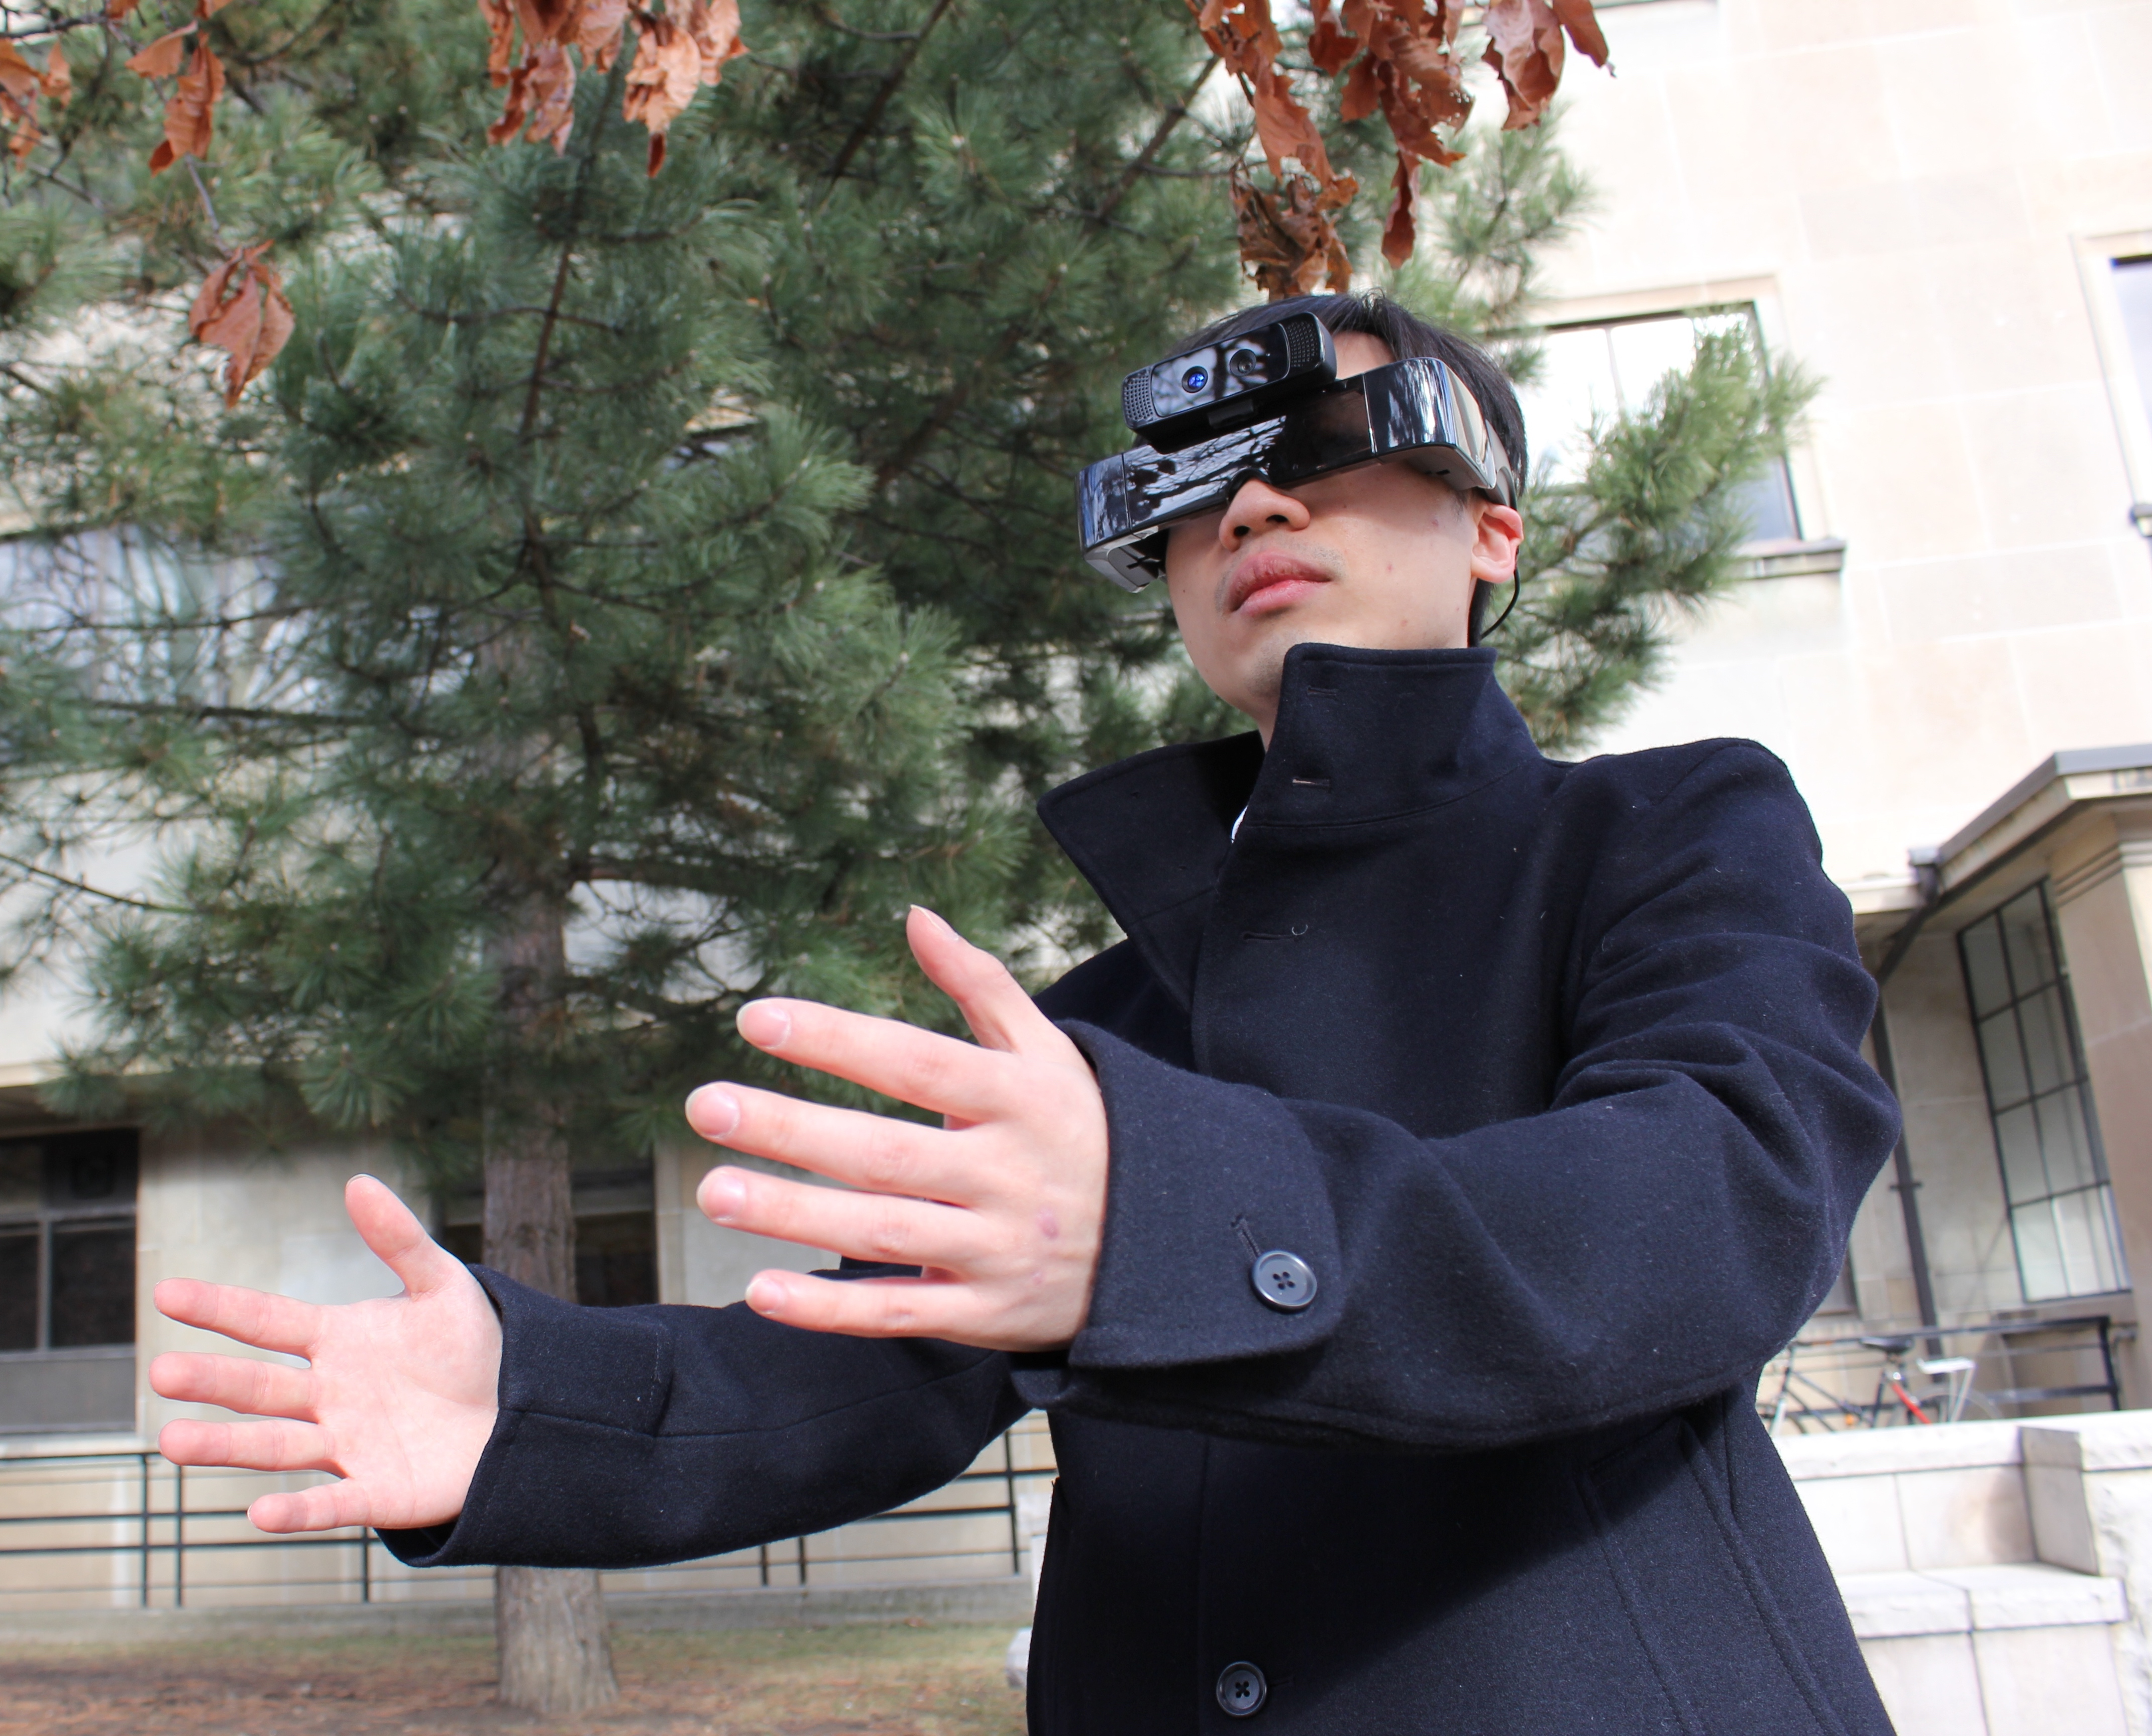
\includegraphics[height=2.8in]{ch7/figures/tree.jpg}

 \caption{Images of the Digital Eye Glass system in the final prototype stage. We can see the fully untethered setup which runs on a battery-powered mobile computer. I was able to perform most of my daily tasks with this setup in both indoor and outdoor settings.}
 \label{fig:prototypes}
\end{figure*}



%%%%========================================================================

% TODO: Need a citation on "life-logging project" 
% I actually didn't get why/how you created prescription for his right eye?  Do you mean HDR or 3D range sensing somehow corrects his vision?  It doesn't make sense.
\begin{figure}
\center
 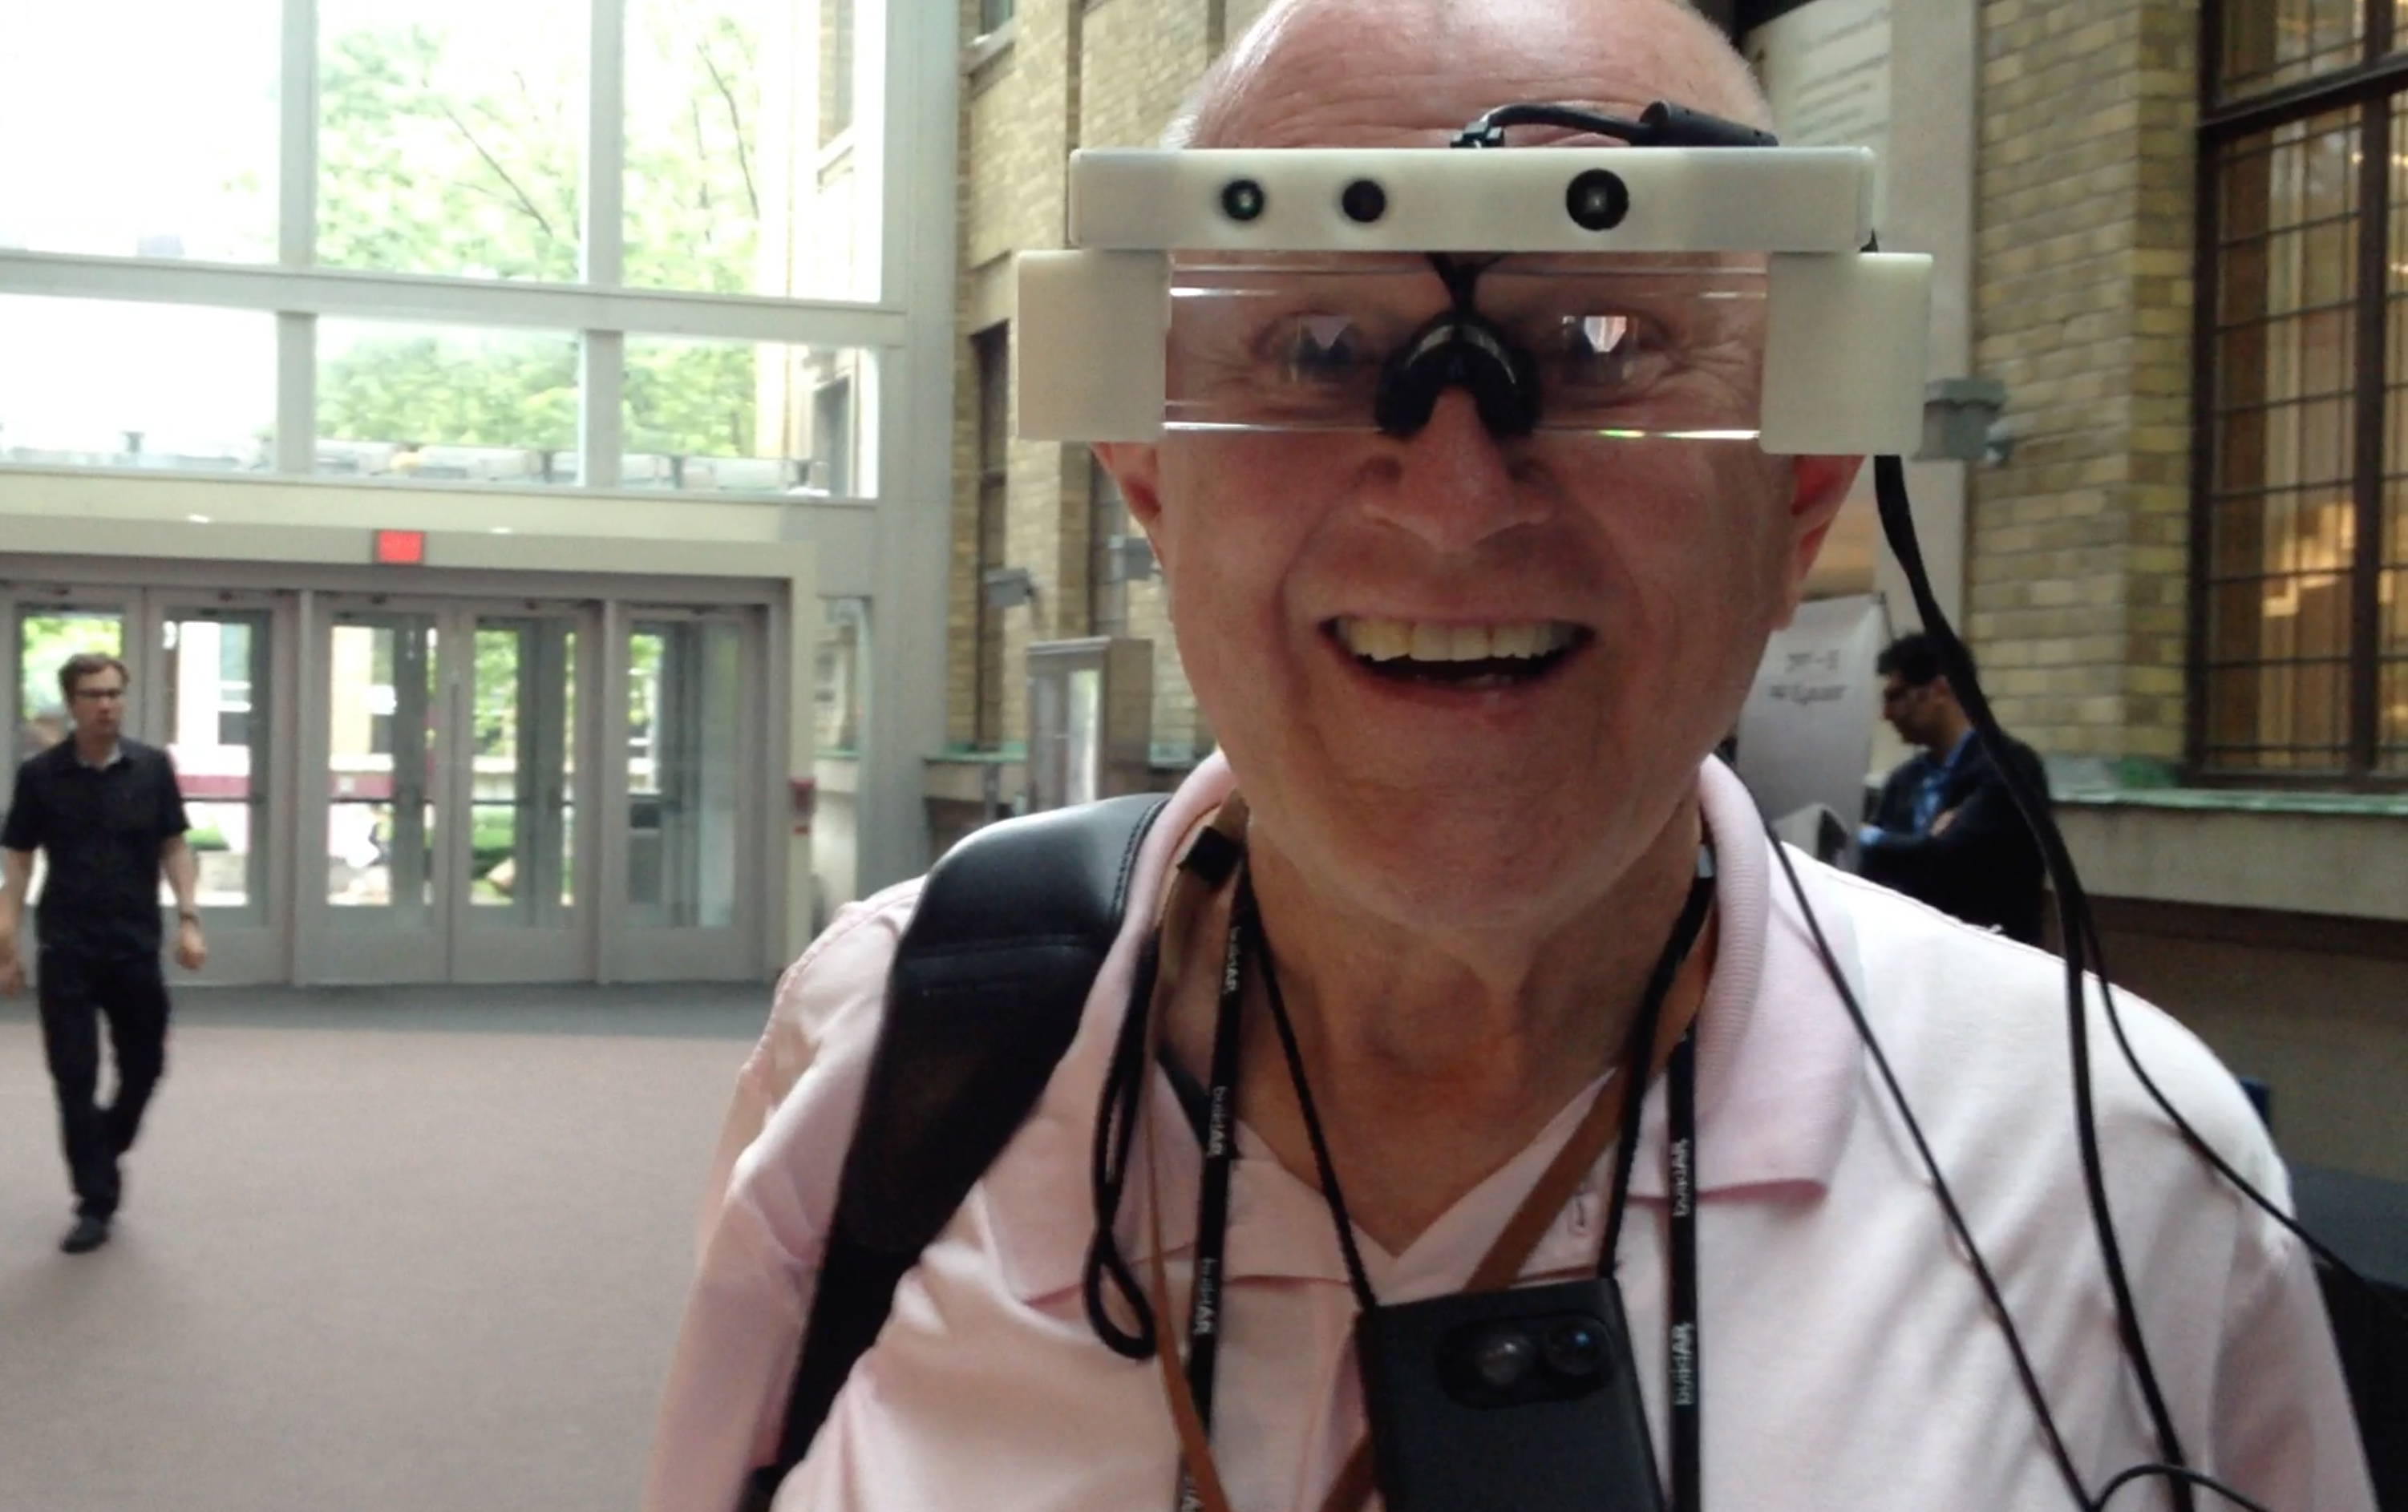
\includegraphics[width=5in]{ch7/figures/GordenBell.jpg}
 \caption{ Gordon Bell, who's a notable scientist and researcher on the life-logging project and received his PhD from MIT, was trying the Digital Eye Glass prototype.  The prototype provided a very delightful experience where he could now see ``better'' than what has otherwise been impossible to achieve with ordinary analog eyeglasses. At the moment he was trying the eyeglasses, he said, ``\textit{You have created the eye formula for my right side (eye)}''. The optics used in the prototype project a clear image onto his retina and he gave me the genuine smile that was truly inspiring.}
 \label{fig:gordanbell}
\end{figure}


%And together, often times, with enough time in wearing the device, often human can adapt to the limitations, such as limited FOV of the camera and forcing the user to 

To summarize, the major contributions of the thesis are outlined as follows: 

% TODO: Here be as technical and thorough as you can.  Read the introduction of every chapter and extract the most important or unique contributions
\begin{itemize}
%Ch2
\item Dynamic Range Management for HDR 3D-Stereo Video
\begin{enumerate}[(I)]
\item Developed a real-time, high-performance HDR video processing system running at 60 fps on FPGAs (and over 60 fps at 1280x720 resolution) for various real-time HDR applications.
\item Verified the robustness of the algorithm and the ability to adapt to rapid changes in lighting  conditions even in the most extreme scenario in TIG welding.  
\item Created a fully functional prototype based on FPGAs with the iCLUT method.
\item Created a fully programmable and flexible pipeline on GPUs with iCLUT and hardware-optimized local contrast enhancement method based on the GPU-accelerated Recursive Filter in Domain Transform.
\item Created a customized firmware that enables the use of 3 exposure settings for handling extreme dynamic cases.
% >>>>>>>>>>>>>>>WL:  What does that mean?  3 exposure settings?  Doesn't every camera do it?  
\item Created a functional DEG which is based on the EyeTap principle for TIG welding purposes.
% >>>>>>>>>>>>>>>WL: What is the EyeTap principle?
\item Demonstrated various use cases, such as remote experts and driving, for the HDR DEG in everyday life.
\end{enumerate}

%Ch 3
\item High Dynamic Range in 3D Depth Sensing Technology
\begin{enumerate}[(I)]
\item Created a method of extending the range of 3D depth-sensing technology with HDR methods and camera calibration.
\item Implemented the one-time optical calibration process which provides alignments for all sensor data.
\item Presented the first 3D-HDR-RGBD data structure which can be used to address limitations in wearable applications in the future.
\item Created a functional prototype which runs the 3-D-HDR algorithm in real-time (\~30fps). 
\end{enumerate}

%Ch 4
\item Gestural Input with Depth Sensors and Machine Learning
\begin{enumerate}[(I)]
\item Implemented a depth sensor based gesture recognition system on a mobile platform with real-time (\~30fps) performance.
\item Attained 96.8\% accuracy in recognition with 4 basic gesture modes.
\end{enumerate}

%Ch 5
\item Social Implications and Applications of DEG. 
\begin{enumerate}[(I)]
\item Explored and discussed the topic of sousveillance and Aliba applications in DEG.
\item Created a framework for the open-source Freeglass project that allows DEG to become a ubiquitous platform for research in wearable computing.  
\end{enumerate}

\end{itemize}

The work presented in this thesis was peer reviewed and published in the following list of 
conferences and copyrighted to IEEE and ACM: 

\begin{itemize}

\item
Raymond Chun Hing Lo, Steve Mann, Jason Huang, Valmiki Rampersad, and Tao Ai. High Dynamic Range (HDR) Video Image Processing for Digital Glass. In Proceedings of the 20th ACM international conference on Multimedia, pages 1477--1480. ACM, 2012.
\cite{lo2012high}

\item
S. Mann, R. Lo, J. Huang, V. Rampersad, and R. Janzen. HDRchitecture: Real-time Stereoscopic HDR imaging for Extreme Dynamic Range. In ACM SIGGRAPH 2012 Emerging Technologies, page 11. ACM, 2012.
\cite{mann2012hdrchitecture}

\item
Steve Mann, Raymond Chun Hing Lo, Kalin Ovtcharov, Shixiang Gu, David Dai, Calvin Ngan, and Tao Ai. Realtime HDR (high dynamic range) Video for EyeTap Wearable Computers, FPGA- based Seeing Aids, and GlassEyes (EyeTaps). In Electrical \& Computer Engineering (CCECE), 2012 25th IEEE Canadian Conference on, pages 1--6. IEEE, 2012.
\cite{mann2012realtime}

\item
Raymond Lo, Valmiki Rampersad, Jason Huang, and Steve Mann. Three dimensional high dynamic range veillance for 3D range-sensing cameras. In Technology and Society (ISTAS), 2013 IEEE International Symposium on, pages 255--265. IEEE, 2013.
\cite{lo2013three}

\item
Raymond Lo, Alexander Chen, Valmiki Rampersad, Jason Huang, Han Wu, and Steve Mann. Augmediated reality system based on 3d camera selfgesture sensing. In Technology and Society (ISTAS), 2013 IEEE International Symposium on, pages 20--31. IEEE, 2013.
\cite{lo2013augmediated}

\item
Steve Mann, Mir Adnan Ali, Raymond Lo, and Han Wu. FreeGlass for developers,`haccessibility', and Digital Eye Glass+ Lifeglogging research in a (sur/sous) veillance society. In Information Society (i-Society), 2013 International Conference on, pages 48�53. IEEE, 2013.
\cite{mann2013freeglass}
\end{itemize}

% IMPORTANT: No do NOT call this an "ongoing" effort - it's complete (you're done, hence PhD defense), but the future directions to explore in AR include. 
% This section needs some citations perhaps.  
% Also be careful about how you approach this section (wording is important); otherwise, you are listing all the weaknesses of your thesis.  It should be more like the future directions
\section{Future Directions in AR}


%%%%========================================================================
%%<This section is slightly vague and does not seem to belong here!   This is more like the future unless you tie it back to the HI principles as explored by your Digital Eye Glass system>>>>>  

Fundamentally, each of the tools created for DEG must follow a set of HI guidelines in order to function with the human. Some principles may seem trivial, such as ``always on" and ``always ready". However, in a wearable computing environment, it is critical that the system can function immediately without cumbersome input devices such as the mouse or the keyboard, or assuming that at the time of use there is access to other machines. The always on, or `power-on-and-ready' mode is critical to DEG especially when one primary purpose of the DEG is a seeing aid. 

Controllability and observability, the two signal paths between the human and machine in the HI principles, are critical. For example, it is often more important to enable the auto-gain with centre-weighted matrices rather than developing a detection algorithm which may have unpredictable outcome even at 1\% detection error rate. That implies that it is very critical for the computer to present information in an intuitive, predictable, or most importantly controllable fashion to the user. Many of the modern electronics such as point-and-shoot cameras today often provide no feedback to users. Any unpredictable behaviours or any sort of automation that requires extensive conscious attention from the human will eventually create user frustration and defeat the purpose of wearable computing.

Furthermore, as high performance computers, sensors, and display hardware become more accessible to researchers, the field of human-computer interaction has growing interest in exploring AR/VR as the new medium for humanistic computing, and a number of studies explored various ways to tightly couple human and the machine~\cite{khundam2015first, biocca2013communication, wright2014using, henrikson2016multi}. Some examples include controller-based or hand free interaction~\cite{Arora:vrSketching:2017}, storytelling and narrative~\cite{henrikson2016multi}, sensory augmentation and amplification~\cite{wright2014using}, telepresence communication~\cite{biocca2013communication,earnshaw2014virtual} with AR/VR recently emerging as the new enabling platform due to the availability of processing power and hardware.

The physical restrictions associated with conventional interfaces, such as panels, controllers, and cameras affixed to the world, are becoming less prominent as interface technology evolves. Assumptions of a static scene and a lab-controlled environment with a limited number of interaction modes often do not apply to real-life wearable computing. This is because the computer is always on and becomes a part of our body and mind in our everyday lives with constantly changing environment and unpredictable situations. 

Designing and building the DEG prototype involved the investigation of several fundamental issues in the practical implementation of Augmented Reality wearable computing devices. Some  notable emerging fields of research include advancement in display technology such as lightfield displays\cite{wetzstein2011layered}, HDR displays \cite{reinhard2010high}, or retinal scanning techniques using laser to create high fidelity, high dynamic range images that also address issues associated with vergence accommodation conflicts \cite{takahashi2008stereoscopic} in typical 3D stereoscopic displays which are used in the current prototypes. On the other hand, low latency tracking is another essential element for an enjoyable wearable computing experience. The ability to add virtual content in the real world can open up many new applications such as wayfinding and virtual guidance. 

Finally, the latency and accuracy of input devices serve an important role in the final interactive experience. In particular, the lack of haptics feedback creates a perceptual issue that degrades the user's experience \cite{yang2016perceptual}~\cite{buchmann2004fingartips}. The ultimate wearable computer in the future, therefore, must address the graphics rendering, tracking, and user input problems holistically, and thus HI principles should be at the core of such a design path.

% TODO: Why don't you just focus on the Future of computing enabled by the translation of the research in this thesis to a commercial development kit.  Introduce the features of the development kit and focus on how they are derived from this thesis (especially Meta 1).  Meta 2 is a group effort, but mention the innovation briefly there.  Focus on what applications and possibilities are enabled by this research development platform.  It's almost a big extension of Ch 5 where you explored social implications, except here it is much more specific and "useful" finally. 
\section{Moving Beyond Research} 

%%This paragraph is fairly vague = and you are emphasizing collaborators here...
%The limited availability of hardware (e.g., the capability of the touch panel, controllers, and other tracking devices). Often times, acquiring the expertise across many fields, ranges from industrial design, computer and electrical engineering, mathematics, physicists, to computer science, can be a very difficult task in research field with limited funding. Fortunately, during the time I was in the lab, I had supports from supervisors as well as many of the collaborators who contributed to various critical technical problems. These collective knowledge, is the key success for the thesis, were many of the difficult challenges can be surfaced and researched on, and together pushing the boundary of the problems.

The continuous effort in advancing the DEG prototype had also bought tremendous amount of interests in the industry. Currently, the work explored in this thesis have been further translated into a development kit that is available for purchase in the market. The release of Google Glass project from Google, the 2 billion dollars acquisition of Oculus Rift (virtual reality platform), 1.4 billion dollars fund raising from Magic Leap, release of Hololens from Microsoft, and release of Meta 2 Developer Kit from Meta had created a strong momentum behind creating the ultimate Augmented Reality (AR) and Virtual Reality (VR) experience. We can expect that in the near future, AR/VR hardware will be commonly available similar to mobile phones today, with significant number of potential applications and implications in our everyday life as shown in Fig.~\ref{fig:futureAR}. 


\begin{figure*}
\center
\begin{subfigure}[b]{3.0in}
\centering
  \includegraphics[height=1.69in]{ch7/figures/future/shopping.png} 
  \caption{Shopping}
  \label{fig:shopping}
\end{subfigure}
\begin{subfigure}[b]{3.0in}
\centering
  \includegraphics[height=1.69in]{ch7/figures/future/3d_visualization.png} 
  \caption{3D Visualization}
  \label{fig:3dvisual}
\end{subfigure}
\begin{subfigure}[b]{3.0in}
\centering
  \includegraphics[width=3.0in]{ch7/figures/future/drawing.png} 
  \caption{3D Drawing}
  \label{fig:3Ddrawing}
\end{subfigure}
\begin{subfigure}[b]{3.0in}
\centering
  \includegraphics[width=3.0in]{ch7/figures/future/architect.png} 
  \caption{Architecture}
  \label{fig:architecture}
\end{subfigure}
\begin{subfigure}[b]{3.0in}
\centering
  \includegraphics[height=1.85in]{ch7/figures/future/medical.png} 
  \caption{Medical Education}
  \label{fig:m_education}
\end{subfigure}
\begin{subfigure}[b]{3.0in}
\centering
  \includegraphics[height=1.85in]{ch7/figures/future/education.png} 
  \caption{Research}
  \label{fig:education}
\end{subfigure}
\caption{Future applications of the Augmediated Digital Eye Glass described in this thesis in our everyday life, ranging from online shopping, 3D visualization in architecture and medicine, to research and beyond (images from http://www.metavision.com/).}
\label{fig:futureAR}
\end{figure*}

% The success or failure of such a synergy would be an existential question for humanity.

In the near future, with embodied humanistic intelligence through the ubiquitous use of the augmediated digital eye glass, there will be a natural synergy between human and machine. While humanity will continue to be constrained and bounded by our own physical and biological limitations, wearable computing technology will continue to advance and transcend significantly beyond our own capabilities or limitations. Inevitably, such a natural machine will form the basis for the true extension of our body and mind, by enabling a new form of superhuman intelligence through the seamless integration of human and machine.
 % Keep this short and just add a series of screenshots - I wonder if you need all these subsections but it may help for those who skim your text.   
%\begin{figure}
%\center
% \includegraphics[width=5in]{ch7/figures/small_meta_1_developer_kit.jpg}
% \caption{Example of Meta 1 Developer Kit. The headset provides the depth sensing solution similar to my original prototypes, and further optimized for close range hand interaction. A field of view extending optics is also embedded in the setup to provide 35 degree FOV, instead of 23 degree FOV in the original setup. By 2015, over 1500 of units were sold and shipped to the customer.}
% \label{fig:meta1}
%\end{figure}

%\begin{figure}
%\center
% \includegraphics[width=5in]{ch7/figures/Meta-Meta-2-Being-Worn-B.jpg}
% \caption{Example of Meta 2 Developer Kit being worn. The headset is developed with a set of sensors, which are capable of seeing 270 degrees with the fisheye cameras, and also seeing 3D information with a depth sensor. The headset also provides a large field of view optics which enables a much more immersive experience for data visualization and such.}
% \label{fig:meta2}
%\end{figure}

%\begin{figure}
%\center
% \includegraphics[width=5in]{ch7/figures/tencent.jpg}
% \caption{Example of Meta 2's hand tracking and physics engine demonstrated on stage. Notice how I can reach out to virtual content and interact with each of the individual virtual cubes in space with my bare hands. The depth sensor on the headset provides real-time hand tracking and also provided a way of interacting with virtual scene based on 3D point cloud's electric force calculation.}
% \label{fig:meta2onstage}
%\end{figure}


